% Template for ICASSP-2021 paper; to be used with:
%          spconf.sty  - ICASSP/ICIP LaTeX style file, and
%          IEEEbib.bst - IEEE bibliography style file.
% --------------------------------------------------------------------------
\documentclass{article}
\usepackage{spconf,amsmath,graphicx}
\usepackage{subcaption}
\usepackage{amsthm}
\usepackage{amsfonts}
\usepackage{enumitem}
\usepackage{amssymb}
\usepackage{xcolor}
%\usepackage{esvect}
\usepackage{url}
\usepackage{graphicx}
\usepackage{subcaption}
\usepackage[ruled,vlined]{algorithm2e}
\usepackage{xcolor}
\usepackage[normalem]{ulem}
\usepackage{amsfonts}
\usepackage{amsmath}
\usepackage{amssymb}
\usepackage{xcolor}
\usepackage{amsthm}
%\usepackage{algorithm}
%\usepackage{algorithmicx}

\newtheorem{definition}{Definition}
\newtheorem{proposition}{Proposition}
\newtheorem{assumption}{Assumption}[section]
\newtheorem{corollary}[assumption]{Corollary}%[section]
\newtheorem{theorem}[assumption]{Theorem}%[section]
\newtheorem{lemma}[assumption]{Lemma}


\DeclareMathOperator{\Unif}{Unif}

\usepackage{hyperref}
\newcommand{\asaf}[1]{{\color{blue}{#1}}}
\newcommand{\asafc}[1]{{\color{blue}{[Asaf: #1]}}}

\newcommand{\A}[0]{\mathcal{A}}
\newcommand{\Var}[0]{\operatorname{Var}}
\newcommand{\SNR}[0]{\text{SNR}}
\newcommand{\E}[0]{\mathbb{E}}

\newcommand{\Cov}[0]{\operatorname{Cov}}
\newcommand{\R}[0]{\mathbb{R}}
% Title.
% ------
\title{Multi-target detection with the generalized method of moments}
%
% Single address.
% ---------------
\name{Ye'Ela Shalit*, Ran Weber*, Asaf Abas*, Shay Kreymer*, and Tamir Bendory\thanks{* These four authors have contributed equally to this work. \newline
S.K. is supported by the Yitzhak and Chaya Weinstein Research Institute for Signal Processing. T.B. is supported in part by NSF-BSF grant no. 2019752, and the Zimin Institute for Engineering Solutions Advancing Better Lives.}}
\address{School of Electrical Engineering, Tel Aviv University, Tel Aviv, Israel}
%
% For example:
% ------------
%\address{School\\
%	Department\\
%	Address}
%
% Two addresses (uncomment and modify for two-address case).
% ----------------------------------------------------------
%\twoauthors
%  {A. Author-one, B. Author-two\sthanks{Thanks to XYZ agency for funding.}}
%	{School A-B\\
%	Department A-B\\
%	Address A-B}
%  {C. Author-three, D. Author-four\sthanks{The fourth author performed the work
%	while at ...}}
%	{School C-D\\
%	Department C-D\\
%	Address C-D}

\begin{document}
%\ninept
%
\maketitle
%
\begin{abstract}
The abstract should appear at the top of the left-hand column of text, about
0.5 inch (12 mm) below the title area and no more than 3.125 inches (80 mm) in
length.  Leave a 0.5 inch (12 mm) space between the end of the abstract and the
beginning of the main text.  The abstract should contain about 100 to 150
words, and should be identical to the abstract text submitted electronically
along with the paper cover sheet.  All manuscripts must be in English, printed
in black ink.
\end{abstract}
%
\begin{keywords}
One, two, three, four, five
\end{keywords}
%
\section{Introduction}
\label{sec:intro}

We study the multi-target detection (MTD) problem of estimating a target signal~\mbox{$x: \{0, \ldots, L-1\} \rightarrow \mathbb{R}$} from a noisy measurement that contains multiple copies of the signal, each randomly translated~\cite{bendory2019multi}, \cite{lan2020multi}, \cite{marshall2020image}, \cite{bendory2021multi}, \cite{kreymer2021two}, \cite{bendory2018toward}. Specifically, let~\mbox{$y: \{0, \ldots, N-1\} \rightarrow \mathbb{R}$} be a measurement of the form
\begin{equation}
\label{eq:model}
y[\ell] = \sum_{i=1}^{p} x[\ell - \ell_i] + \varepsilon[\ell],
\end{equation}
where \mbox{$\{\ell_i\}_{i=1}^{p} \in \{L + 1, \ldots, N-L\}$} are arbitrary translations, and~$\varepsilon[\ell]$ is i.i.d. Gaussian noise with zero mean and \mbox{variance~$\sigma^2$}.

The translations and the number of occurrences of~$x$ in~$y$ are unknown. Figure~\ref{fig:measurements} presents an example of a measurement~$y$ at different signal-to-noise ratios (SNRs). We define~\mbox{$\text{SNR} := \frac{\|x\|_\text{F}^2}{L \sigma^2}$}, where~$L$ is the length of~$x$ (in pixels), and~$\sigma^2$ is the noise variance.

\begin{figure*}[!tb]
	\begin{subfigure}[ht]{0.30\textwidth}
		\centering
		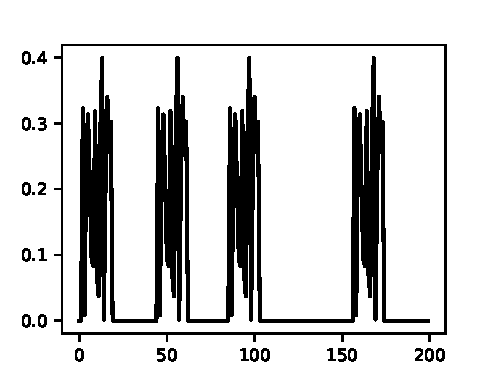
\includegraphics[width=\columnwidth]{figures/y_clean.pdf}
		\caption{No noise.}
	\end{subfigure}
	\hfill
	\begin{subfigure}[ht]{0.30\textwidth}
		\centering
		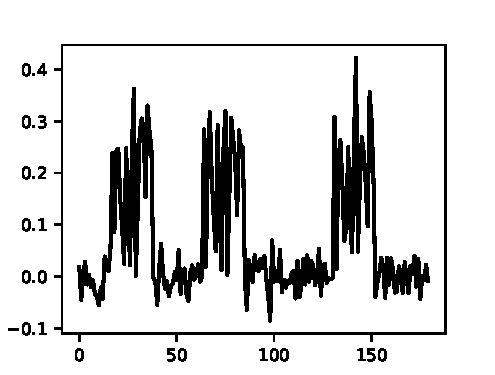
\includegraphics[width=\columnwidth]{figures/y_SNR50.pdf}
		\caption{$\text{SNR} = 50$.}
	\end{subfigure}
	\hfill
	\begin{subfigure}[ht]{0.30\textwidth}
		\centering
		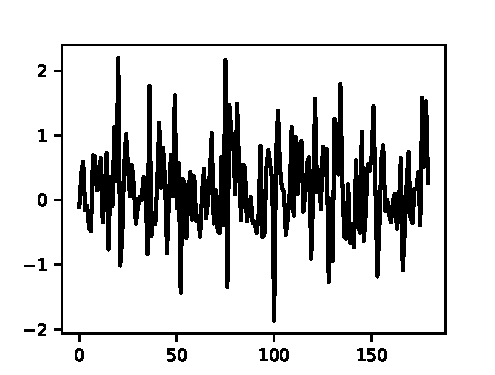
\includegraphics[width=\columnwidth]{figures/y_SNR01.pdf}
		\caption{$\text{SNR} = 0.1$.}
	\end{subfigure}
	\caption{Three measurements~$y$ from~(\ref{eq:model}) at different noise levels: no noise (left);~\mbox{$\text{SNR} = 50$} (middle);~\mbox{$\text{SNR} = 0.1$} (right). Each measurement contains multiple copies of the target signal in arbitrary locations. In this work, our goal is to estimate the target signal directly from~$y$. We focus on the low SNR regime~(e.g., panel~(c)) in which the signal occurrences are swamped by the noise, and the locations of the signal occurrences cannot be detected reliably.}
\label{fig:measurements}
\end{figure*}

The MTD model arises in several scientific applications, such as passive radar~\cite{gogineni2017passive}, astronomy~\cite{schulz1993multiframe}, motion deblurring~\cite{levin2006blind}, and system identification~\cite{abed1997blind}. In particular, it serves as mathematical abstraction of the cryo-electron microscopy~(\mbox{cryo-EM}) technology for macromolecular structure determination~\cite{henderson1995potential},~\cite{nogales2016development},~\cite{bai2015cryo}. In a \mbox{cryo-EM} experiment \cite{frank2006three}, biological macromolecules suspended in a liquid solution are rapidly frozen into a thin ice layer. An electron beam then passes through the sample, and a two-dimensional tomographic projection is recorded. Importantly, the \mbox{2-D} location and \mbox{3-D} orientation of particles within the ice are random and unknown. This measurement, called \textit{micrograph}, is affected by high noise levels and the optical configuration of the microscope. This transformation is typically modeled as a convolution of the model~(\ref{eq:model}) with a point spread function, whose Fourier transform is called contrast transfer function~(CTF)~\cite{heimowitz2020reducing}, \cite{erickson1971measurement}.

In the current analysis workflow of \mbox{cryo-EM} data \cite{bendory2020single}, \cite{scheres2012relion}, \cite{punjani2017cryosparc}, the~\mbox{2-D} projections are first detected and extracted from the micrograph, and later rotationally and translationally aligned to reconstruct the~\mbox{3-D} molecular structure. This approach fails for small molecules, which induce low contrast, and thus low SNR. This makes them difficult to detect and align~\cite{bendory2018toward}, \cite{henderson1995potential}, \cite{bendory2020single}, \cite{aguerrebere2016fundamental}, rendering current \mbox{cryo-EM} algorithmic pipeline ineffective. For example, in the limit~\mbox{$\text{SNR} \rightarrow 0$}, reliable detection of signals' locations within the measurement is impossible~\cite[Proposition~3.1]{bendory2018toward}.

The MTD model was devised in \cite{bendory2018toward} in order to study the recovery of small molecules directly from the micrograph, below the current detection limit of \mbox{cryo-EM}~\cite{henderson1995potential},~\cite{d2021current}. An autocorrelation analysis technique (see Section~\ref{subsec:ac}) was implemented to recover \mbox{low-resolution}~\mbox{3-D} structures from noiseless simulated data under a simplified model. Autocorrelation analysis consists of finding an image that best explains the empirical autocorrelations of the measurement. For any noise level, those autocorrelations can be estimated to any desired accuracy for sufficiently large~$N$. Computing the autocorrelations is straightforward and requires only one pass over the data, which is advantageous for massively large datasets, such as \mbox{cryo-EM} datasets~\cite{bendory2020single}. As such, autocorrelation analysis provides an attractive alternative to other computational methods, such as maximum likelihood estimation, which is intractable for the MTD problem~\cite{lan2020multi}.


The method of moments is a classical statistical inference technique, tracing back to 1894~\cite{pearson1894contributions}. This work expand n similar estimation to method of moments which is based upon an autocorrelations analysis~\cite{bendory2019multi}, which is described in detail in Section~\ref{subsec:relations}. The estimator results in a set of parameters whose autocorrelations agree with the empirical autocorrelations of the signal~$y$, by minimizing a {least-squares} (LS) objective. {For computing} the autocorrelations, a single pass through the signal is required. This {single-pass requirement} stands in contrast to main-stream parameter estimation techniques, such as  maximum likelihood {estimation}, which usually {iterates} over the data. The method


This work studies the application of the estimator \textit{generalized method of moments} (GMM) and its application to the MTD problem. The GMM theory, which was first introduced in~\cite{Hansen1982},  shows that the GMM provides {an} optimal estimator, in compare to others weighted LS objective function (or an equivalent, such as autocorrelations). As shown in previous work, the GMM estimator suggests a significant improvement in the estimation error~\cite{abas2021generalized}.

\section{Mathematical framework}
\label{sec:math}
\subsection{Autocorrelation analysis}
\label{subsec:ac}
The autocorrelation of order~$q$ of a random signal~\mbox{$z \in \mathbb{R}^{N}$} is defined as
\begin{equation}
A_z^q[\ell_1, \ldots, \ell_{q-1}] := \mathbb{E}_z\Big[\frac{1}{N^2} \sum_{i \in \mathbb{R}^2} z[i] z[i + \ell_1] \cdots z[i + \ell_{q-1}]\Big],
\end{equation}
where~$\ell_1, \ldots, \ell_{q-1}$ are integer shifts. Indexing out of bounds is zero-padded, that is,~\mbox{$z[i] = 0$} out of the range~\mbox{$\{0, \ldots, {N-1}\}$}. In this work, we use the first three autocorrelations which are explicitly given by
\begin{align}
\label{eq:ac1}
A_z^1 &= \mathbb{E}_z \left[\frac{1}{N} \sum_{i \in \mathbb{Z}} z\left[i\right] \right], \\
\label{eq:ac2}
A_z^2\left[\ell\right] &= \mathbb{E}_z \left[\frac{1}{N} \sum_{i \in \mathbb{Z}} z\left[i\right] z\left[i + \ell\right] \right], \\
\label{eq:ac3}
A_z^3\left[\ell_1, \ell_2\right] &= \mathbb{E}_z \left[\frac{1}{N} \sum_{i \in \mathbb{Z}} z\left[i\right] z\left[i + \ell_1\right] z\left[i + \ell_2\right] \right].
\end{align}
As~$N$ grows indefinitely, the empirical autocorrelations of~$z$ almost surely (a.s.) converge to the population autocorrelations of~$z$:
\begin{equation}
\lim_{N \rightarrow \infty} \frac{1}{N} \sum_{i \in \mathbb{Z}^2} z[i] z[i + \ell_1] \cdots z[i + \ell_{q-1}] \stackrel{\text{a.s.}}{=}A_z^q[\ell_1, \ldots, \ell_{q-1}].
\end{equation}

Our goal is to relate the autocorrelations of the measurement with the target signal~$x$. In particular, the first-order autocorrelation is defined as
\begin{equation}
\label{eq:AM1}
A_{y}^1 := \frac{1}{N} \sum_{i \in \mathbb{Z}} y[i].
\end{equation}
This is the mean of the measurement. The second-order autocorrelation of~$y$, \mbox{$A_{y}^2: \mathbb{Z} \rightarrow \mathbb{R}$}, is defined by
\begin{equation}
\label{eq:AM2}
A_{y}^2 [\ell_1] := \frac{1}{N} \sum_{i \in \mathbb{Z}} y[i] y[i + \ell_1],
\end{equation}
and the third-order autocorrelation~\mbox{$A_{y}^3: \mathbb{Z} \times \mathbb{Z} \rightarrow \mathbb{R}$} by
\begin{equation}
\label{eq:AM3}
A_{y}^3 [\ell_1, \ell_2] := \frac{1}{N} \sum_{i \in \mathbb{Z}} y[i] y[i + \ell_1] y[i + \ell_2].
\end{equation}


\subsection{Autocorrelations under the well-separated model}
\label{subsec:relations}
We first discuss the \mbox{well-separated} case of the MTD problem, which was studied in~\cite{bendory2019multi}. In this case, we assume that each signal in the measurement~$y$ is separated by at least a full signal length from its neighbors. Specifically, we assume that
\begin{equation}
\label{eq:sep}
|\ell_{i_1} - \ell_{i_2}| \ge 2L - 1, \quad \text{ for all } i_1 \ne i_2.
\end{equation}

%Figure~\ref{fig:Micrograph_shifts}(a) presents an example of a measurement obeying the separation condition~(\ref{eq:sep}).
To compute the third-order autocorrelation~(\ref{eq:AM3}), we compute the product of~$y$ with its two shifts. Importantly, for~\mbox{$\ell$-s} in the range
\begin{equation}
\label{eq:set_L}
\mathcal{L} = \{0, \ldots, {L - 1}\},
\end{equation}
any given occurrence of~$x$ in~$y$ is only ever correlated with itself, and never with another occurrence.

In~\cite{bendory2019multi}, it was shown that under the separation condition~(\ref{eq:sep}), for any fixed level of noise~$\sigma^2$, density~$\gamma$ and signal length~$L$, in the limit~\mbox{$N \rightarrow \infty$} we have that
\begin{align}
\label{eq:well_separated_1st}
A_{y}^1 &\stackrel{\text{a.s.}}{=} \gamma A_{x}^1, \\
\label{eq:well_separated_2nd}
A_{y}^2 [\ell_1] &\stackrel{\text{a.s.}}{=} \gamma A_{x}^2 [\ell_1] + \sigma^2\delta[\ell_1], \\
\label{eq:well_separated_3rd}
A_{y}^3 [\ell_1, \ell_2] &\stackrel{\text{a.s.}}{=} \gamma A_{X} [\ell_1, \ell_2] \nonumber \\&+ \gamma S_1 \sigma^2 (\delta[\ell_1] + \delta[\ell_2] + \delta[\ell_1 - \ell_2]),
\end{align}
\asafc{What is $S_1$ above?}
for~$\ell_1, \ell_2 \in \mathcal{L}$ (defined in~(\ref{eq:set_L})), where
\begin{equation}
\label{eq:delta}
\delta[\ell] = \begin{cases} 1 \text{ if } \ell = \vec{0}, \\ 0 \text{ otherwise}, \end{cases}
\end{equation}
is the Kronecker delta function. Here,~$\gamma$ is the density of the target images in the measurement and is defined by
\begin{equation}
\label{eq:gamma}
\gamma = p \frac{L}{N}.
\end{equation}
Next, we introduce the notations for the second and third autocorrelations:
\begin{gather*}
	 \A_y^2 := [A_y^2[\ell
	] ]_{\ell=0}^{L-1},
	\\
	\A_x^2 := [A_x^2[\ell
	]+ \sigma^2 \delta[\ell]]_{\ell=0}^{L-1},
	\\
	\A_y^3 := [A_y^3[\ell_1, \ell_2]]_{\ell_1,\ell_2=0}^{L-1},
	\\
	\A_x^3 := [A_x^3[\ell_1, \ell_2] + \gamma S_1 \sigma^2 (\delta[\ell_1] + \delta[\ell_2] + \delta[\ell_1 - \ell_2])]_{\ell_1,\ell_2=0}^{L-1}
\end{gather*}
Notice, $\A_y^3$ and~$\A_x^3$ are treated as vectors.

As such,~\mbox{(\ref{eq:well_separated_1st}) -~(\ref{eq:well_separated_3rd})} relate the autocorrelations of the measurement with those of the target signal~$x$. Moreover, the signal $x$ can be identified from its autocorrelations, and thus, potentially, also from the autocorrelations of the measurement. In~\cite{bendory2019multi}, it was shown that~$\gamma$ (respectively~$\sigma$) can be estimated from the first- and second-order autocorrelations of the measurement if~$\sigma$ (respectively~$\gamma$) is known. In particular, if~$\gamma$ and~$\sigma$ are known (or are reliably estimated), we can provably determine the signal from the measurement's autocorrelations. Previous works~\cite{bendory2019multi}, \cite{lan2020multi}, \cite{marshall2020image}, \cite{bendory2021multi}, \cite{kreymer2021two} demonstrated successful signal and image estimations. Importantly, the aforementioned relations between the autocorrelations of~$M$ and~$F$ do not directly depend on the location of individual signal occurrences in the measurement, but only through the density parameter~$\gamma$. Therefore, detecting the signal occurrences is not a prerequisite for signal recovery, and thus signal recovery is possible even in very low SNR regimes.

\subsection{Signal recovery from autocorrelations}

\section{Generalized method of moments}
\label{gmm}
\subsection{The GMM framework}\label{gmm:framwork}

In its most simplified form, the GMM generalizes~\eqref{Eq-2-2} by replacing the LS objective with a weighted LS. In particular, a specific choice of weights guarantees favorable asymptotic statistical properties, such as {the} minimal asymptotic variance of the estimation error.

Let us define the \textit{moment function}, $f(\theta, y)\colon \Theta \times \R^r \to \R^q$. The moment function needs to be chosen such that its expectation value is zero only at a single point $\theta=\theta_0$. Namely,
\begin{equation}\label{Eq-GMM-1}
	\E\left[f(\theta,y)\right] = 0 \quad \text{if and only if} \quad \theta = \theta_0.
\end{equation}
We refer to~\eqref{Eq-GMM-1} as the \textit{uniqueness of the parameter set} condition. The moment function must satisfy the uniqueness condition and a few additional regularity conditions (which can be found in~\cite{Hansen1982, abas2021generalized}). This flexibility enables the GMM to be applied to a wide range of problems, such as subspace estimation~\cite{Fan2018}.

In order to define the moment function for the MTD, we first define the $i$-th observation from the signal~$y$ as follow:
\begin{equation}
	y_i := [y[i],\ldots, y[i+L]].
\end{equation}
The moment function~$f(\cdot)$ should fulfil \eqref{Eq-GMM-1} using the defined samples. The natural choice of ~$f(\cdot)$ is
\begin{equation} \label{Eq-GMM-2}
	f(x,\gamma,y_i) :=
	\begin{bmatrix}
		&\gamma A_x^1 - A_{y_i}^1\\
		&\A_x^2 - \A_{y_i}^2 \\
		&\A_x^3 - \A_{y_i}^3
	\end{bmatrix}
\end{equation}



The estimated sample moment function is the average of~$f$ over~$N$ observations:
\begin{equation}\label{Eq-2-5}
	g_N(\theta) = \frac{1}{N} \sum_{i=1}^N f(\theta, y_i) = \begin{bmatrix}
		&\gamma A_x^1 - A_{y}^1\\
		&\A_x^2 - \A_{y}^2 \\
		&\A_x^3 - \A_{y}^3
	\end{bmatrix}.
\end{equation}
The GMM estimator is defined as the minimizer of the weighted LS expression,
\begin{equation} \label{Eq-2-1}
	\hat{\theta}_N = \arg\min_{\theta \in \Theta} \ g_N(\theta)^T W_N g_N(\theta).
\end{equation}
Here, $W_N$ is a fixed positive semi-definite (PSD) matrix. Note that the LS estimator~\eqref{Eq-2-2} is a special case of~\eqref{Eq-2-1}.

\subsection{Large Sample Properties}\label{gmm:large}

Before presenting the statistical properties of the GMM, we fix notation. We denote by $\overset{p}{\to}$ and $\overset{d}{\to}$ convergence in  probability and in distribution, respectively. Let
\begin{equation} \label{eqn:cov_mat_S}
	S := \lim_{N\to \infty}\Cov\left[\sqrt{N}g_N(\theta_0)\right],
\end{equation}
be the covariance matrix of the estimated sample moment function~\eqref{Eq-2-5} at the ground truth~$\theta_0$. We denote by $\{W_N\}_{N=1}^\infty$ a sequence of PSD matrices which converges almost surely to a positive definite (PD) matrix~$W$. Finally, the expectation of the Jacobian of the moment function at the ground truth~$\theta_0$ is denoted by $G_0 = \E\left[\partial f(\theta_0, y) / \partial \theta^T\right]$.

%Following~\cite{Hansen1982}, the large sample properties of the GMM estimator under the uniqueness of the parameter set~\eqref{Eq-2-4} are \tamir{as follows.}

The large sample properties of the GMM estimator, were derived in~\cite{Hansen1982}, and are presented in the following theorem.

\begin{theorem}\label{Thm-2-6}
	Under the uniqueness of the parameter set~\eqref{Eq-2-4}, and {the} regularity conditions {\ref{As-Ap1-1*}-\ref{As-Ap1-8*} of Appendix~\ref{Ap-1}}, the GMM estimator satisfies:
	\begin{enumerate}[label={\Alph*}.]
		\item  \label{Thm-2-2}
		\textnormal{(Consistency)} $\hat{\theta}_N \overset{p}{\to} \theta_0$.

		\item \label{Thm-2-3} \textnormal{(Asymptotic normality)}
		\[\sqrt{N} ( \hat{\theta}_N - \theta_0) \overset{d}{\to} \mathcal{N}(0, M S M^T ),\] where $M =[G_0^T W  G_0]^{-1} G_0^T  W$.

		\item \label{Thm-2-5} \textnormal{(Optimal choice of a weighting matrix)} The minimum asymptotic variance of $\hat{\theta}_N$ is given by $(G_0^T S^{-1} G_0)^{-1}$ and is attained by $W = S^{-1}$.
	\end{enumerate}
\end{theorem}
Theorem~\ref{Thm-2-6} provides a matrix~$W$ {that} guarantees a minimal asymptotic variance of the estimator’s error.

The covariance matrix~$S$ {of~\eqref{eqn:cov_mat_S}, which plays a central role in Theorem~\ref{Thm-2-6},} is required to be a PD matrix. Therefore, the moment function must be chosen so that~$S$ is full-rank. In this work, we noticed that if we remove the repeating entries of~$f$ (that appear due to the inherent symmetries of the autocorrelations), the covariance is indeed full rank (although, in some cases, ill-conditioned).

It is important to note that in practice, the ground truth~$\theta_0$ is unknown a priori, so we cannot use the optimal weighting matrix. A common heuristic is to replace~\eqref{Eq-2-1} with an iterative scheme, which is named iterative GMM.
\asaf{For our choice of the moment function~\eqref{Eq-GMM-2}, it is enough to apply the covariance on the empirical part,
	\begin{equation}\label{Eq-2-7}
		\Cov[g(\theta)] = \Cov\left[\left[A_{y_i}^1;\A_{y_i}^2;\A_{y_i}^3\right]\right].
	\end{equation}
	The covariance depends solely on the observations~$\{y_i\}_{i=1}^N$, not on the input of the parameter set~$\theta$. Therefore, in a single pass one can compute the moments estimators~\eqref{Eq-2-6} and the optimal covariance for~\eqref{Eq-2-3}.
}

\section{Numerical experiments}
\label{sec:numerical}

The paper title (on the first page) should begin 1.38 inches (35 mm) from the
top edge of the page, centered, completely capitalized, and in Times 14-point,
boldface type.  The authors' name(s) and affiliation(s) appear below the title
in capital and lower case letters.  Papers with multiple authors and
affiliations may require two or more lines for this information. Please note
that papers should not be submitted blind; include the authors' names on the
PDF.

\section{Conclusion}
\label{sec:conclusion}



\vfill\pagebreak

\bibliographystyle{IEEEbib}
\bibliography{references}

\end{document}
